\chapter{Uvod}
Projekt FERSAT, koji se od 2018. godine provodi na Fakultetu elektrotehnike i računarstva, uključuje izradu, lansiranje i korištenje jednog nanosatelita CubeSat. Satelit u izradi dimenzija je približno 10 cm x 10 cm x 10 cm, volumena jedne litre i ne teži od 4/3 kilograma, što ga svrstava u skupinu satelita formata CubeSat 1U \cite{fersat_stranica_projekta}. Očekivani životni vijek satelita je 3 godine, a bit će postavljen u Zemljinoj orbiti na visini između 500 i 600 kilometara. Planirani korisni teret \engl{payload} FERSAT-a podijeljen je na tri podsustava:

\begin{itemize}
	\item kamera za snimanje površine Zemlje i zemaljskog horizonta,
	\item detektori svjetla u vidljivom i ultraljubičastom dijelu spektra za mjerenje svjetlosnog onečišćenja i debljine stupca ozona,
	\item komunikacijski sustav u radijskom X-pojasu (10.45 GHz) za prijenos podataka na Zemlju.
\end{itemize}

Radom korisnog tereta upravlja \textit{Payload Data Handler} (PDH) računalo. Zadaća je PDH računala prikupiti podatke iz senzorskog podsustava i kamere, pohraniti ih u trajnu memoriju \engl{non-volatile memory} te poslati te podatke na Zemlju korištenjem komunikacijskog podsustava. Kao PDH računalo odabran je mikrokontroler STM32L471VGT6 proizvođača ST Microelectronics.

Za rad ostalih podsustava satelita koji nisu direktno vezani uz koristan teret (npr. upravljanje položajem satelita, slanje telemetrijskih podataka na Zemlju) brine se \textit{Command and Data Handler} (CDH) računalo. CDH računalo također upravlja napajanjem korisnog tereta i šalje naredbe PDH računalu. Komunikacija CDH i PDH računala odvija se korištenjem sučelja CAN (\textit{Controller Area Network}). Konkretno CDH računalo u trenutku pisanja ovog teksta još nije odabrano.
    
Slika \ref{fig:fersat_blok} prikazuje blok dijagram cijelog sustava. U okviru ovog rada razvijena je programska potpora PDH računala za upravljanje kamerom i \textit{flash} memorijom.

\begin{figure}[H]
	\centering
	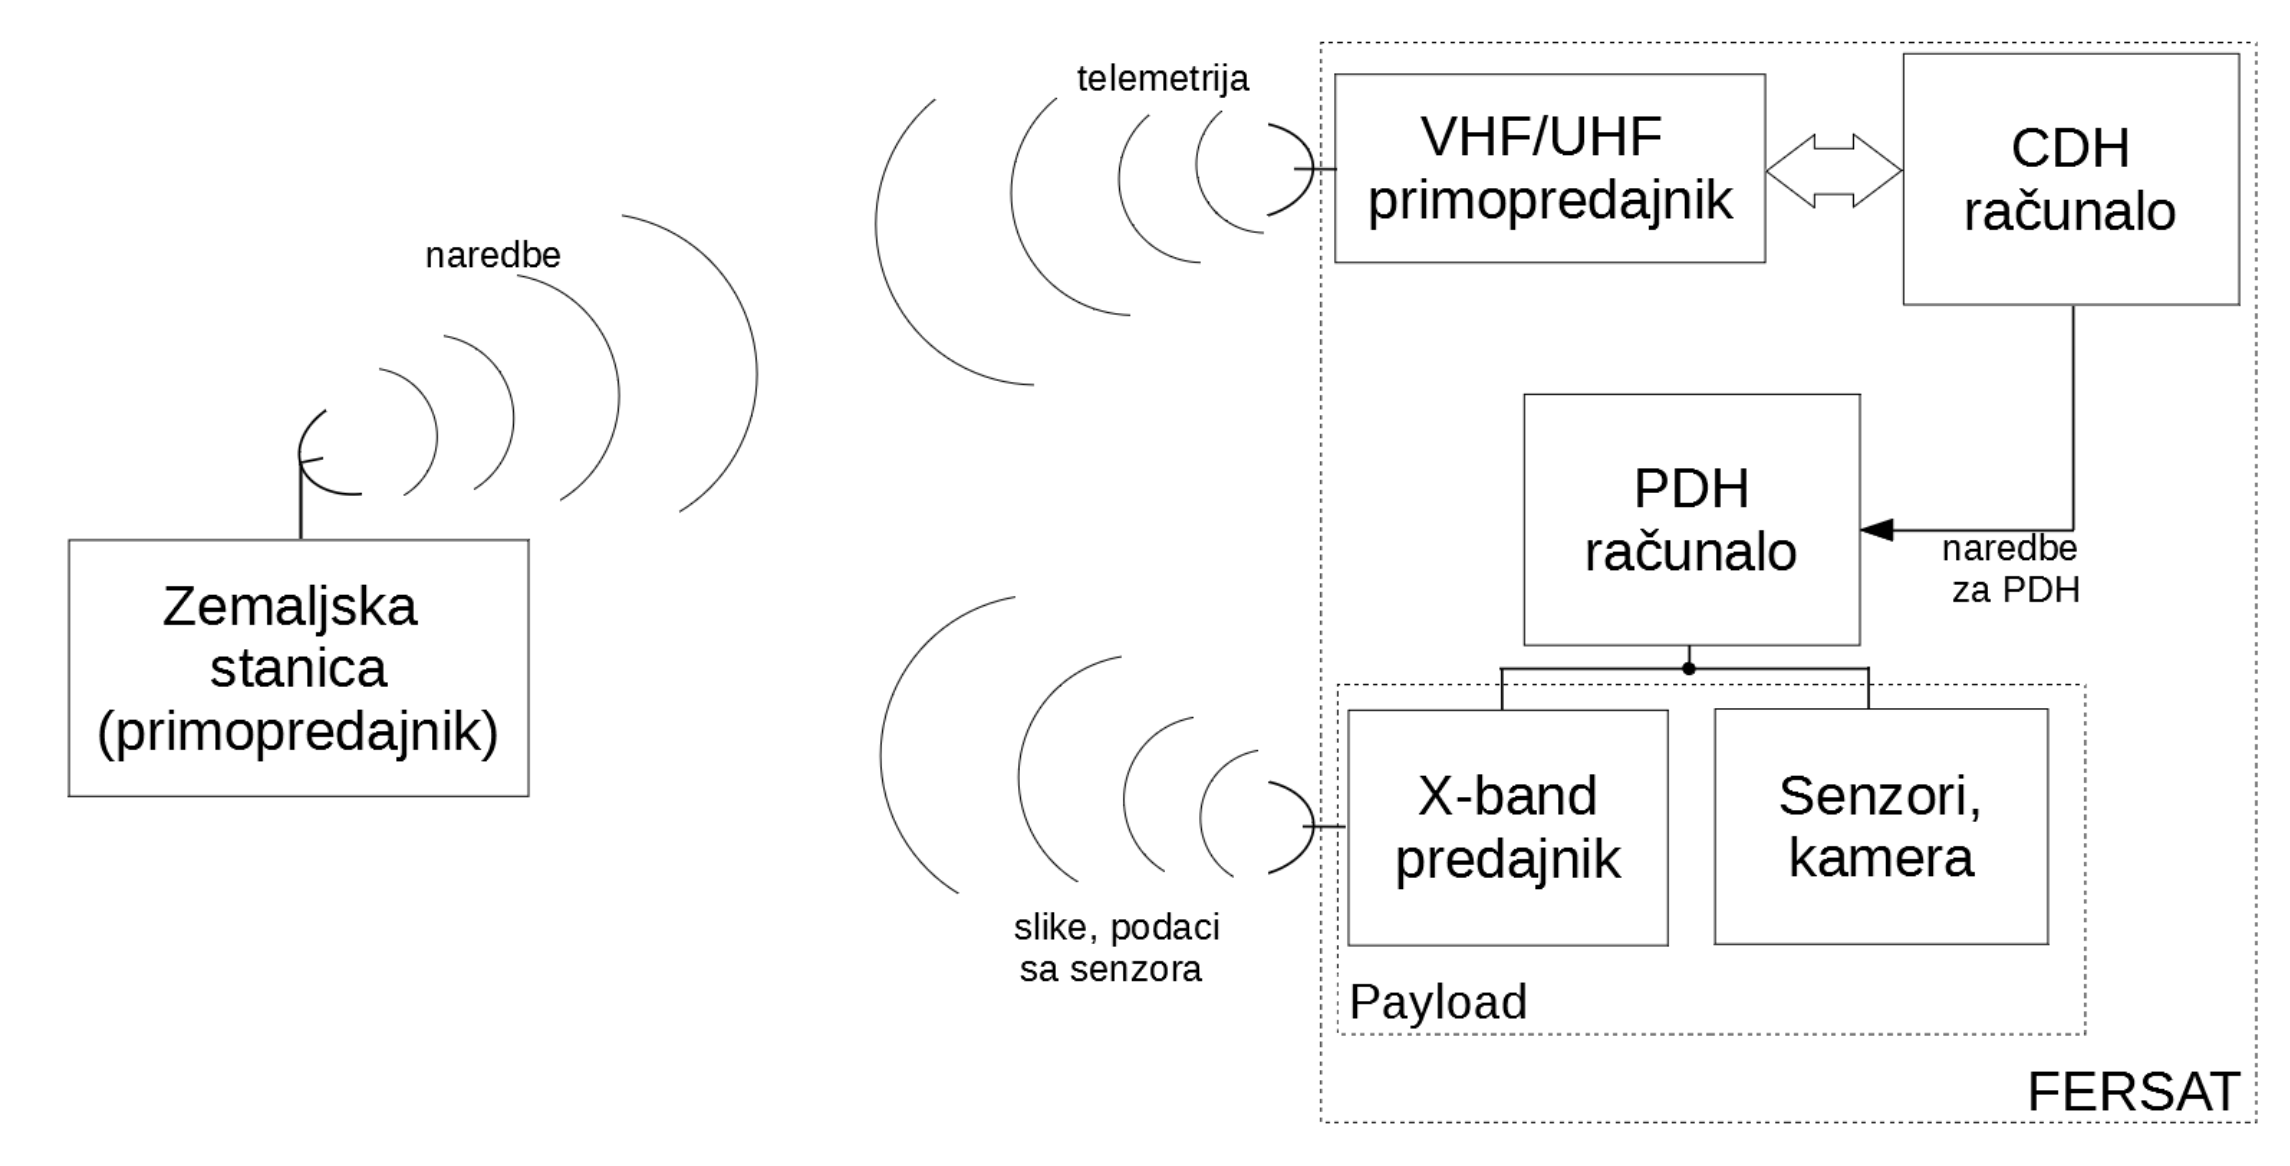
\includegraphics[width=\textwidth]{fersat_blok_dijagram.png}
	\caption{Blok dijagram FERSAT-a i komunikacija sa zemaljskom postajom \cite{diplomski_goran_petrak}}
	\label{fig:fersat_blok}
\end{figure}

Sustav za upravljanje kamerom se sastoji od Arducam Mini 5MP Plus kamere. Upravljanje kamerom se sastoji od konfiguracije kamere i samog korištenja kamere, odnosno slikanja i spermanja slike. Konfiguracija kamere je nužna kako bi se ispravno podesili parametri trajanja ekspozicije, pojačanje i formata u kojem se slika želi spremiti.

Slanjem određenog signala na sklop za kameru može se uslikati slika, a nakon slikanja slika se spremi na vlastiti međuspremnik kamere. Cilj je spremljenu kameru pročitati iz međuspremnika kamere i spremiti ju na \textit{flash} memoriju koja se nalazi na pločici PDH-a, gdje može biti spremljena dok se ne zatraži slanje slike preko X-band predajnika na Zemlju.

\textit{Flash} memorija, osim što služi za pohranu slike, služi i za pohranu podataka sa drugih senzora. Ona prima i šalje podatke ovisno o poslanoj naredbi putem SPI komunikacije sa mikrokontrolerom.

Upravljačko sklopovlje PDH računala se sastoji od STM32F471VGT6 mikrokontrolera, spomenute vanjske \textit{flash} memorije, konektora za povezivanje s ostalim dijelovima sustava (uključujući i konektor za povezivanje s kamerom), sustava za napajanje, upravljačkog sklopovlja za CAN komunikaciju i sklopa za kontrolu izvođenja programa (engl. \textit{watchdog}) \cite{zavrsni_filip_juric}. Izgled tiskane pločice upravljačkog sklopovlja PDH računala prikazan je na slikama \ref{fig:PDH_PCB_1} i \ref{fig:PDH_PCB_2}. Konektor X1 služi za povezivanje sustava sa kamerom.

\begin{figure}[H]
	\centering
	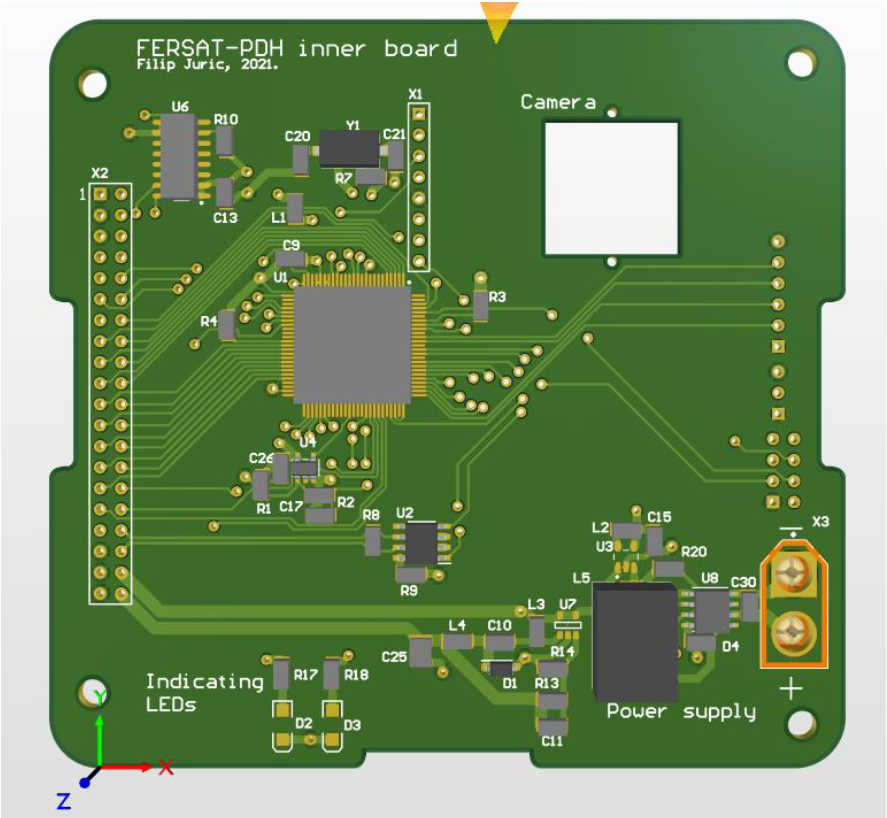
\includegraphics[height= 10 cm]{PDH_PCB_1.PNG}
	\caption{Prikaz gornje strane tiskane pločice upravljačkog sklopovlja PDH računala \cite{zavrsni_filip_juric}}
	\label{fig:PDH_PCB_1}
\end{figure}

\begin{figure}[H]
	\centering
	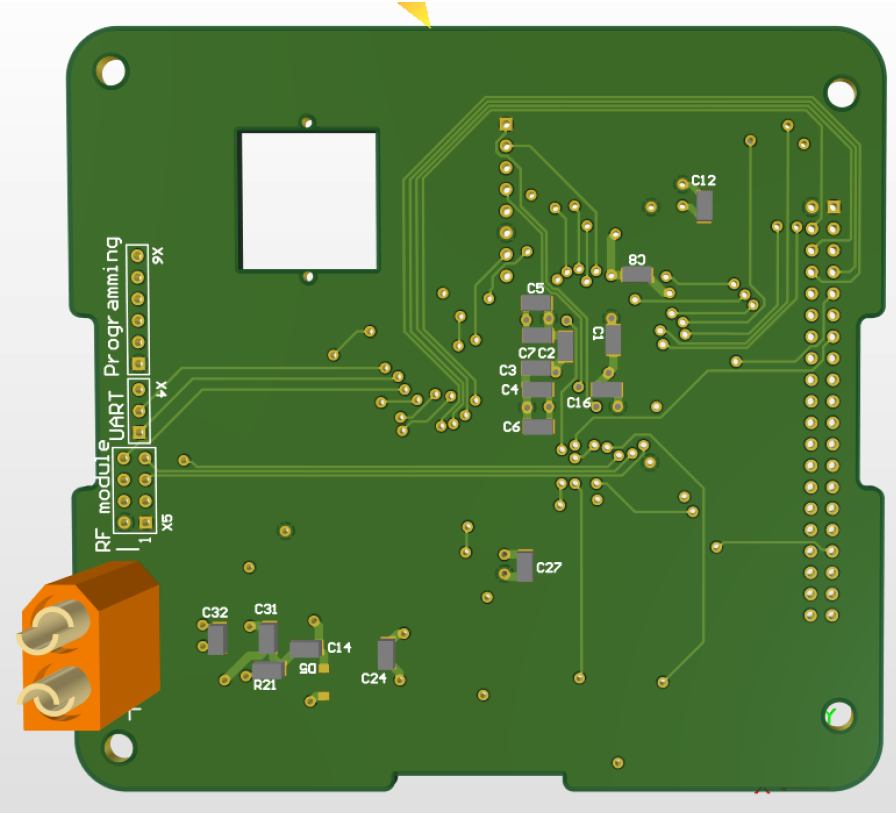
\includegraphics[height= 10 cm]{PDH_PCB_2.PNG}
	\caption{Prikaz donje strane tiskane pločice upravljačkog sklopovlja PDH računala \cite{zavrsni_filip_juric}}
	\label{fig:PDH_PCB_2}
\end{figure}

Programska podrška za PDH računalo već je razvijena \cite{diplomski_goran_petrak}. Međutim, u međuvremenu je došlo do promjene izbora mikrokontrolera PDH računala, te je stoga postojeću programsku podršku bilo potrebno prilagoditi trenutačnom sklopovlju.

S obzirom na prirodu ovog završnog projekta, gdje je naglasak bio na prilagođavanju postojeće programske podrške, u ovom radu će biti raspravljeni izazovi i razlike do kojih je došlo tijekom prilagođavanja programske podrške. U poglavlju 2 dan je detaljan opis I\textsuperscript{2}C komunikacije, te su istaknute razlike između starog i novog sklopovlja koje su bile ključne za prilagođavanje programske podrške. Na isti način opsani su SPI komunikacija i DMA prijenos u poglavlju x. Detaljan pregled razvijene programske podrške dan je u poglavlju y, gdje je opisana integracija programske podrške za kameru i \textit{flash} memorija u FreeRTOS operacijski sustav za rad u stvarnom vremenu.